\section{Convolutional Neural Network}
Some real world application of AI, such as image recognition, naturally work with an input space that is locally structured.
Convolutional Neural Networks (CNNs) are a type of neural network architecture that is particularly well-suited for processing data with a 2D structure, 
such as images.

Similarly to FFNNs, the idea for CNNs has some biological inspiration, as they are loosely based on the structure of the visual cortex in animals.
Neurons are organized in a hierarchical manner, with each layer processing increasingly complex features of the input image, starting from simple edges and 
textures in the early layers to more complex shapes and objects in the deeper layers.

If we were to use a standard FFNN for processing images, we would need to flatten the 2D image into a 1D vector, which would result in a loss
of spatial information and a large number of parameters to learn, making the model prone to overfitting.
CNNs are designed on 2 principles that allow them to effectively process images while keeping the number of parameters manageable:
\begin{itemize}
    \item \textbf{Local Connectivity}: each neuron in a CNN is connected only to a small region of the layer before it;
    \item \textbf{Parameter Sharing}: the same set of weights is shared across different spatial locations in the input image.
    This allows the model to learn translation-invariant filters, while also significantly reducing the number of parameters to learn.
\end{itemize}

\subsection{Convolution}
Convolutional Neural Networks basically replace general matrix multiplications with convolution operations in at least one layer of the network.

\subsubsection*{1-D Convolution}
Even though CNNs are typically used for processing 2D images, it's important to remember that the convolution operation can be applied to any type of data, including 1D sequences (e.g., time series, text)
\begin{figure}[H]
    \centering
    \definecolor{kernelblue}{RGB}{100,180,220}
\definecolor{boxgray}{RGB}{220,220,220}
\definecolor{outputgray}{RGB}{200,200,200}

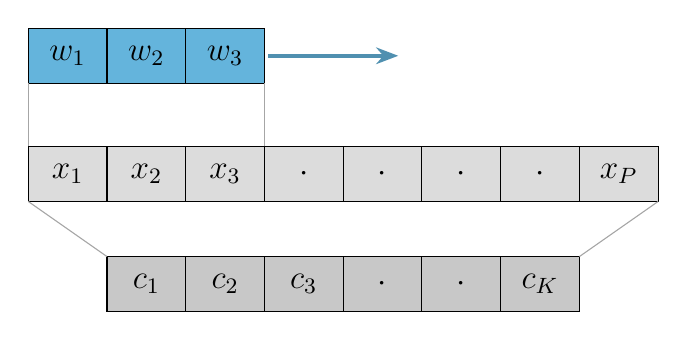
\begin{tikzpicture}[
    kernelcell/.style={draw, fill=kernelblue, minimum width=1cm, minimum height=0.7cm, font=\large},
    inputcell/.style={draw, fill=boxgray, minimum width=1cm, minimum height=0.7cm, font=\large},
    outputcell/.style={draw, fill=outputgray, minimum width=1cm, minimum height=0.7cm, font=\large},
]
% Kernel row at y=2.5
% Each cell is 1cm wide, anchor=center, placed at x = 0,1,2
\node[kernelcell] (k1) at (0.0, 2.5) {$w_1$};
\node[kernelcell] (k2) at (1.0, 2.5) {$w_2$};
\node[kernelcell] (k3) at (2.0, 2.5) {$w_3$};

% Arrow pointing right from kernel
\draw[-{Stealth[length=8pt]}, line width=1.5pt, color=kernelblue!80!black]
    (2.55, 2.5) -- (4.2, 2.5);

% Input row at y=1.0  (8 cells, x=0..7)
\node[inputcell] (x1) at (0.0, 1.0) {$x_1$};
\node[inputcell] (x2) at (1.0, 1.0) {$x_2$};
\node[inputcell] (x3) at (2.0, 1.0) {$x_3$};
\node[inputcell]      at (3.0, 1.0) {$\cdot$};
\node[inputcell]      at (4.0, 1.0) {$\cdot$};
\node[inputcell]      at (5.0, 1.0) {$\cdot$};
\node[inputcell]      at (6.0, 1.0) {$\cdot$};
\node[inputcell] (xP) at (7.0, 1.0) {$x_P$};

% Lines from kernel bottom corners down to input top corners
\draw[gray!70, thin] (-0.5, 2.15) -- (-0.5, 1.35);
\draw[gray!70, thin] (2.5,  2.15) -- (2.5,  1.35);

% Output row at y=-0.4  (6 cells, x=1..6, so centered below input)
\node[outputcell] (c1) at (1.0, -0.4) {$c_1$};
\node[outputcell] (c2) at (2.0, -0.4) {$c_2$};
\node[outputcell] (c3) at (3.0, -0.4) {$c_3$};
\node[outputcell]      at (4.0, -0.4) {$\cdot$};
\node[outputcell]      at (5.0, -0.4) {$\cdot$};
\node[outputcell] (cK) at (6.0, -0.4) {$c_K$};

% Lines from input bottom corners to output top corners
\draw[gray!70, thin] (-0.5, 0.65) -- (0.5, -0.05);
\draw[gray!70, thin] (7.5,  0.65) -- (6.5, -0.05);

\end{tikzpicture}
    \caption{Example of a 1D convolution operation.}
    \label{fig:1D-convolution}
\end{figure}
Given the example shown in the figure \ref{fig:1D-convolution}, we can express the convolution operation as follows:
$$ c_1 = w_1 x_1 + w_2 x_2 + w_3 x_3 $$
$$ c_2 = w_1 x_2 + w_2 x_3 + w_3 x_4 $$
And so on, where $w_i$ are the weights of the filter and $x_i$ are the input values.

\subsubsection*{2-D Convolution}
In the case of 2D convolution, the input is a 2D image, and the convolution operation is performed by sliding a small filter (also called kernel) across the image and computing the dot product between the filter and the local region of the image.
Formally, the output of a convolution operation for a given input image $I$ and filter $K$ is defined as:
$$ (I * K)(x, y) = \sum_{i} \sum_{j} I(x+i, y+j) \cdot K(i, j) $$
where $ * $ denotes the convolution operation.

\begin{figure}[H]
    \centering
    \definecolor{kernelblue}{RGB}{100,180,220}
\definecolor{boxgray}{RGB}{220,220,220}
\definecolor{outputgray}{RGB}{200,200,200}
\definecolor{highlightblue}{RGB}{60,140,200}
\definecolor{receptiveyellow}{RGB}{255,215,70}

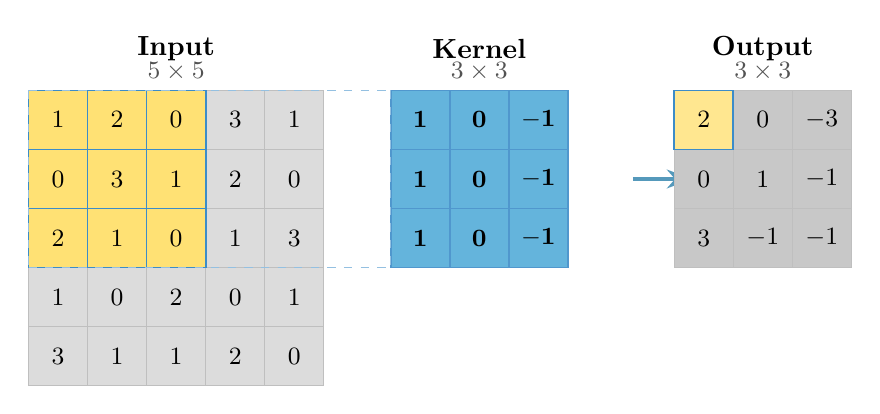
\begin{tikzpicture}

\def\S{0.75}
\def\H{0.375}

\tikzset{
  IC/.style={draw=gray!50, fill=boxgray,
    minimum width=\S cm, minimum height=\S cm, inner sep=0},
  AC/.style={draw=highlightblue, fill=receptiveyellow!75,
    minimum width=\S cm, minimum height=\S cm, inner sep=0, line width=0.6pt},
  KC/.style={draw=highlightblue!90, fill=kernelblue,
    minimum width=\S cm, minimum height=\S cm, inner sep=0, line width=0.6pt},
  OC/.style={draw=gray!50, fill=outputgray,
    minimum width=\S cm, minimum height=\S cm, inner sep=0},
  OA/.style={draw=highlightblue, fill=receptiveyellow!60,
    minimum width=\S cm, minimum height=\S cm, inner sep=0, line width=0.6pt},
}

% ── INPUT 5×5 with real values ───────────────────────────────────
% Values row by row (r=0 top … r=4 bottom)
\def\inputvals{
  {1,2,0,3,1},
  {0,3,1,2,0},
  {2,1,0,1,3},
  {1,0,2,0,1},
  {3,1,1,2,0}
}

\foreach \r in {0,...,4}{
  \foreach \c in {0,...,4}{
    \node[IC] at (\c*\S, -\r*\S) {};
  }
}
% Receptive field highlight
\foreach \r in {0,1,2}{
  \foreach \c in {0,1,2}{
    \node[AC] at (\c*\S, -\r*\S) {};
  }
}
% Numeric labels
\foreach \r/\rowvals in {
  0/{1,2,0,3,1},
  1/{0,3,1,2,0},
  2/{2,1,0,1,3},
  3/{1,0,2,0,1},
  4/{3,1,1,2,0}
}{
  \foreach \c/\val in {0/1,1/2,2/0,3/3,4/1}{} % dummy, use explicit below
}

% Explicit cell values (row, col, value)
% Row 0
\node[font=\small] at (0*\S, 0*\S) {1};
\node[font=\small] at (1*\S, 0*\S) {2};
\node[font=\small] at (2*\S, 0*\S) {0};
\node[font=\small] at (3*\S, 0*\S) {3};
\node[font=\small] at (4*\S, 0*\S) {1};
% Row 1
\node[font=\small] at (0*\S,-1*\S) {0};
\node[font=\small] at (1*\S,-1*\S) {3};
\node[font=\small] at (2*\S,-1*\S) {1};
\node[font=\small] at (3*\S,-1*\S) {2};
\node[font=\small] at (4*\S,-1*\S) {0};
% Row 2
\node[font=\small] at (0*\S,-2*\S) {2};
\node[font=\small] at (1*\S,-2*\S) {1};
\node[font=\small] at (2*\S,-2*\S) {0};
\node[font=\small] at (3*\S,-2*\S) {1};
\node[font=\small] at (4*\S,-2*\S) {3};
% Row 3
\node[font=\small] at (0*\S,-3*\S) {1};
\node[font=\small] at (1*\S,-3*\S) {0};
\node[font=\small] at (2*\S,-3*\S) {2};
\node[font=\small] at (3*\S,-3*\S) {0};
\node[font=\small] at (4*\S,-3*\S) {1};
% Row 4
\node[font=\small] at (0*\S,-4*\S) {3};
\node[font=\small] at (1*\S,-4*\S) {1};
\node[font=\small] at (2*\S,-4*\S) {1};
\node[font=\small] at (3*\S,-4*\S) {2};
\node[font=\small] at (4*\S,-4*\S) {0};

% Input label — moved higher
\node[font=\normalsize\bfseries]        at (1.5, 0.90) {Input};
\node[font=\small, text=gray!65!black]  at (1.5, 0.62) {$5 \times 5$};

% ── KERNEL 3×3 with real values ──────────────────────────────────
% kernel values: [[1,0,-1],[1,0,-1],[1,0,-1]]  (vertical edge detector)
\def\KX{4.6}

\foreach \r in {0,1,2}{
  \foreach \c in {0,1,2}{
    \node[KC] at (\KX+\c*\S, -\r*\S) {};
  }
}
% Kernel values
\node[font=\small\bfseries] at (\KX+0*\S, 0*\S) { 1};
\node[font=\small\bfseries] at (\KX+1*\S, 0*\S) { 0};
\node[font=\small\bfseries] at (\KX+2*\S, 0*\S) {$-$1};
\node[font=\small\bfseries] at (\KX+0*\S,-1*\S) { 1};
\node[font=\small\bfseries] at (\KX+1*\S,-1*\S) { 0};
\node[font=\small\bfseries] at (\KX+2*\S,-1*\S) {$-$1};
\node[font=\small\bfseries] at (\KX+0*\S,-2*\S) { 1};
\node[font=\small\bfseries] at (\KX+1*\S,-2*\S) { 0};
\node[font=\small\bfseries] at (\KX+2*\S,-2*\S) {$-$1};

% Kernel label — moved higher
\node[font=\normalsize\bfseries]        at (\KX+0.75, 0.90) {Kernel};
\node[font=\small, text=gray!65!black]  at (\KX+0.75, 0.62) {$3 \times 3$};

% Top horizontal
\draw[highlightblue!55, dashed, thin] (-\H, \H) -- (\KX-\H, \H);
% Bottom horizontal
\draw[highlightblue!55, dashed, thin] (-\H,-2*\S-\H) -- (\KX-\H,-2*\S-\H);
% Left vertical (RF side)
\draw[highlightblue!55, dashed, thin] (-\H, \H) -- (-\H,-2*\S-\H);
% Right vertical (kernel side)
\draw[highlightblue!55, dashed, thin] (\KX-\H, \H) -- (\KX-\H,-2*\S-\H);

\draw[-{Stealth[length=9pt]}, line width=1.8pt, color=kernelblue!85!black]
    (7.30, -\S) -- (8.05, -\S);

\def\OX{8.2}

\foreach \r in {0,1,2}{
  \foreach \c in {0,1,2}{
    \node[OC] at (\OX+\c*\S, -\r*\S) {};
  }
}
% Highlight active output cell c_{1,1}
\node[OA] at (\OX+0*\S, 0*\S) {};

% Output values
\node[font=\small] at (\OX+0*\S, 0*\S)  { 2};
\node[font=\small] at (\OX+1*\S, 0*\S)  { 0};
\node[font=\small] at (\OX+2*\S, 0*\S)  {$-$3};
\node[font=\small] at (\OX+0*\S,-1*\S)  { 0};
\node[font=\small] at (\OX+1*\S,-1*\S)  { 1};
\node[font=\small] at (\OX+2*\S,-1*\S)  {$-$1};
\node[font=\small] at (\OX+0*\S,-2*\S)  { 3};
\node[font=\small] at (\OX+1*\S,-2*\S)  {$-$1};
\node[font=\small] at (\OX+2*\S,-2*\S)  {$-$1};

% Output label — moved higher
\node[font=\normalsize\bfseries]        at (\OX+0.75, 0.90) {Output};
\node[font=\small, text=gray!65!black]  at (\OX+0.75, 0.62) {$3 \times 3$};

\end{tikzpicture}


    \caption{Example of a 2D convolution operation.}
    \label{fig:2D-convolution}
\end{figure}
In the figure \ref{fig:2D-convolution}, we can see an example of a 2D convolution operation, where the input image is a $5 \times 5$ grid of pixel values, and the filter is a $3 \times 3$ kernel with specific values. 
The output of the convolution operation is a new $3 \times 3$ grid of values, where each value is computed as the dot product between the kernel and the corresponding local region of the input image.

\subsection{Inside a CNN}
A CNN is typically composed of several stacked layers, each performing a specific operation on the input data. 
Usually, low-level layers of the network learn to extract simple local features (e.g., edges, textures), while deeper layers learn to combine these features 
into more complex and abstract representations (e.g., shapes, objects).

Different types of layers can be used in a CNN, each one serving a specific purpose. In the following sections, we will briefly describe the most common types of layers used in CNNs.

\subsubsection{Convolution Layer}
The convolution layer is the core building block of a CNN, where the convolution operation is performed to extract features from the input data.
Each layer consists of a set of filters (or kernels), covering a specific region of the input image, called the receptive field. 
These filters are applied across the entire input image, through the process of convolution, to produce a feature map that highlights the presence 
of specific features in the input image.

Differently from what was happening with feature extraction, where filters were designed manually, 
in CNNs the network learns the best filters for the task at hand through backpropagation and gradient descent, 
allowing it to automatically discover relevant features from the data.

It's important to note that the convolution layer has some hyperparameters that can be tuned to control the behavior of the convolution operation, such as:
\begin{itemize}
    \item \textbf{Kernel Size}: the size of the filter (e.g., $3 \times 3$, $5 \times 5$) that determines the size of the receptive field and the amount 
    of local information captured by the convolution operation.
    \item \textbf{Stride}: the step size with which the filter is moved across the input image. For example, a stride of 1 means that
    the filter is applied at every possible position, while a stride of 2 means that the filter is applied at every other position, effectively downsampling the output feature map.
    \item \textbf{Padding}: the output feature map produced by the convolution operation is smaller than the input image, due to the size of the kernel.
    To preserve the spatial dimensions of the input image, we can add padding (e.g., zeros) around the borders of the input image before applying the convolution operation.
\end{itemize}

\subsubsection{Non-Linearity Layer}
After the convolution layer, a non-linearity layer is typically applied to introduce non-linear transformations to the feature maps.
This is usually done using activation functions such as ReLU (Rectified Linear Unit), similar to what we have seen in FFNNs.
The non-linearity layer allows the network to learn more complex and non-linear relationships between the input data and the output.

\subsubsection{Pooling Layer}
The pooling layer is used to downsample the feature maps produced by the convolution layer, reducing their spatial 
dimensions while retaining the most important information.

This is typically done using operations such as max pooling or average pooling, which respectively take the maximum or average 
value from a local region of the feature map, to produce a smaller output feature map.

This also helps to create the translation invariance property of CNNs, as the exact position of the features in the input image becomes less important after pooling.

\subsection{Different Architectures}
In this section, we will briefly describe some of the most popular CNN architectures that have been proposed in the literature, each one with its own unique design and characteristics.

\subsubsection{LeNet (1998)}
The LeNet architecture, proposed in 1998, is one of the earliest CNN architectures and was designed for handwritten digit recognition.
\begin{figure}[H]
    \centering
    \input{chapters/03-cnn/tikz/LeNet.tex}
    \caption{LeNet architecture.}
    \label{fig:LeNet}
\end{figure}
It follows a simple architecture pattern, using 2 convolutional layers (C1 and C3), each followed by a pooling layer (S2 and S4).
Finally, 2 fully connected layers (C5 and F6) are used to produce the final output, which is a probability distribution over the 10 possible digit classes (0-9).

\subsubsection{AlexNet (2012)}
Introduced for the 2012 ImageNet Large Scale Visual Recognition Challenge (ILSVRC), AlexNet significantly evolved the foundational 
concepts of LeNet. 
While it retained a similar structural logic, it scaled the complexity to 5 convolutional layers and 3 fully connected layers.
\begin{figure}[H]
    \centering
    \input{chapters/03-cnn/tikz/AlexNet.tex}
    \caption{AlexNet architecture.}
    \label{fig:AlexNet}
\end{figure}
This architecture marked a turning point for deep learning. 
By dramatically outperforming existing methods on ImageNet, AlexNet demonstrated the power of deep convolutional networks and
guided the research community towards deeper and more complex architectures.

Beyond its performance, AlexNet fundamentally changed how features were perceived. 
Previously, image processing relied on hand-crafted descriptors like SIFT or GIST paired with classifiers such as SVMs. 
AlexNet proved that an end-to-end trained CNN could automatically learn hierarchical features that were far more robust. 
Researchers soon discovered that these learned representations were highly transferable, outperforming manual features in diverse applications—including object detection, 
segmentation, and natural language processing.

\subsubsection{Zeiler and Fergus (2013)}
After the success of AlexNet, a natural question was: how can we understand what the network has learned?

The Zeiler and Fergus architecture, proposed in 2013, introduced a method for visualizing and understanding the features learned by deep convolutional networks. 
This approach involved deconvolutional networks, that allowed to invert the operations of a CNN, visualizing the activations of the different layers and understanding which features were being captured by the network.
\begin{figure}[H]
    \centering
    \usetikzlibrary{decorations.markings,calc,positioning,arrows,shapes.geometric,arrows.meta,matrix}
\usetikzlibrary{3d,perspective}


% colors centralized in setup.tex

\begin{tikzpicture}[font=\small,scale=1, every node/.style={outer sep=0pt, inner sep=0pt, align=center, fill=white}, w/.style={minimum width=#1},h/.style={minimum height=#1},s/.style={minimum size=#1}, eu/.style={shorten >=#1},ed/.style={shorten <=#1},line join=round,isometric view, canvas is xy plane at z=0]

\tikzset{>={Latex[length=1.5mm, width=1.25mm]}}

  \foreach \i in {0,0.5,1,1.5} \foreach \j in {0,0.5,1,1.5} {
    \pgfmathparse{ifthenelse(\i<1 && \j>=1, "dlyellow!40", ifthenelse(\i>=1 && \j>=1, "dlgreen!25", ifthenelse(\i<1 && \j<1, "dlsky!40", "dlred!25")))}
    \fill[\pgfmathresult,draw=dlgray] (\i,\j) rectangle (\i+0.5,\j+0.5);
  }
  \draw[dlgray] (0,0,0) rectangle (2, 2,0);

% Bars
\node[draw, fill=dlgray, w=.15cm, h=.4cm, anchor=south] at (.25,1.75,0) {};
\node[draw, fill=white, w=.15cm, h=.6cm, anchor=south] at (.75,.75,0) {};
\node[draw, fill=white, w=.15cm, h=.3cm, anchor=south] at (1.25,.25,0) {};
\node[draw, fill=dlgray, w=.15cm, h=.6cm, anchor=south] at (1.75,1.25,0) {};


% 2*2 matrix
\begin{scope}[xshift=2cm, yshift=2cm]
\foreach \i in {0,0.5} 
            \foreach \j in {0,0.5} {
                \pgfmathparse{ifthenelse(\i==0 && \j==0.5, "dlyellow!40", 
                               ifthenelse(\i==0.5 && \j==0.5, "dlgreen!25", 
                               ifthenelse(\i==0 && \j==0, "dlsky!40", 
                               "dlred!25")))}
                % Center the smaller grid above the larger one
                \fill[\pgfmathresult,draw=dlgray] (\i+0.5,\j+0.5,1) rectangle (\i+1,\j+1,1);
            }
        \draw[dlgray] (0.5,0.5,1) rectangle (1.5,1.5,1);

% Bars
\node[draw, fill=dlgray, w=.15cm, h=.4cm, anchor=south] at (0.5+.8,0.5+.75,0) {};
\node[draw, fill=white, w=.15cm, h=.5cm, anchor=south] at (0.5+.2,0.5+.25,0) {};
\node[draw, fill=white, w=.15cm, h=.3cm, anchor=south] at (0.5+.75,0.5+.25,0) {};
\node[draw, fill=dlgray, w=.15cm, h=.3cm, anchor=south] at (0.5+.25,0.5+.75,0) {};
\end{scope}

%---------------------------------------

\begin{scope}[xshift=5cm, yshift=-5cm]
  \foreach \i in {0,0.5,1,1.5} \foreach \j in {0,0.5,1,1.5} {
    \pgfmathparse{ifthenelse(\i<1 && \j>=1, "dlyellow!40", ifthenelse(\i>=1 && \j>=1, "dlgreen!25", ifthenelse(\i<1 && \j<1, "dlsky!40", "dlred!25")))}
    \fill[\pgfmathresult,draw=dlgray] (\i,\j) rectangle (\i+0.5,\j+0.5);
  }
  \draw[dlgray] (0,0,0) rectangle (2, 2,0);

% Bars
\node[draw, fill=white, w=.15cm, h=.05cm, anchor=south] at (0.25,0.25,0) {};
\node[draw, fill=white, w=.15cm, h=.05cm, anchor=south] at (1.25,0.75,0) {};
\node[draw, fill=white, w=.15cm, h=.05cm, anchor=south] at (1.75,0.75,0) {};
\node[draw, fill=white, w=.15cm, h=.15cm, anchor=south] at (1.25,1.2,0) {};
\node[draw, fill=white, w=.15cm, h=.05cm, anchor=south] at (1.25,1.75,0) {};
\node[draw, fill=white, w=.15cm, h=.05cm, anchor=south] at (1.75,1.75,0) {};
\node[draw, fill=white, w=.15cm, h=.05cm, anchor=south] at (.75,1.75,0) {};
\node[draw, fill=white, w=.15cm, h=.2cm, anchor=south] at (.25,1.25,0) {};

\node[draw, fill=dlgray, w=.15cm, h=.4cm, anchor=south] at (.25,1.75,0) {};
\node[draw, fill=white, w=.15cm, h=.6cm, anchor=south] at (.7,.75,0) {};
\node[draw, fill=white, w=.15cm, h=.3cm, anchor=south] at (1.25,.25,0) {};
\node[draw, fill=dlgray, w=.15cm, h=.6cm, anchor=south] at (1.75,1.25,0) {};
% 2*2 matrix
\begin{scope}[xshift=2cm, yshift=2cm]
\foreach \i in {0,0.5} 
            \foreach \j in {0,0.5} {
                \pgfmathparse{ifthenelse(\i==0 && \j==0.5, "dlyellow!40", 
                               ifthenelse(\i==0.5 && \j==0.5, "dlgreen!25", 
                               ifthenelse(\i==0 && \j==0, "dlsky!40", 
                               "dlred!25")))}
                % Center the smaller grid above the larger one
                \fill[\pgfmathresult,draw=dlgray] (\i+0.5,\j+0.5,1) rectangle (\i+1,\j+1,1);
            }
        \draw[dlgray] (0.5,0.5,1) rectangle (1.5,1.5,1);

% Bars
\node[draw, fill=white, w=.15cm, h=.4cm, anchor=south] at (0.5+.8,0.5+.75,0) {};
\node[draw, fill=white, w=.15cm, h=.5cm, anchor=south] at (0.5+.2,0.5+.25,0) {};
\node[draw, fill=white, w=.15cm, h=.4cm, anchor=south] at (0.5+.75,0.5+.25,0) {};
\node[draw, fill=white, w=.15cm, h=.6cm, anchor=south] at (0.5+.25,0.5+.75,0) {};
\end{scope}
\end{scope}

\begin{scope}[xshift=4cm, yshift=-1cm]
\foreach \i in {0,0.5,1,1.5} 
  \foreach \j in {0,0.5,1,1.5} {
    \pgfmathparse{ifthenelse(
      (\i==0 && \j==1.5) || (\i==1 && \j==0) || (\i==0.5 && \j==.5) || (\i==1.5 && \j==1),
      "dlgray!20", "dlgray"
    )}
    \fill[\pgfmathresult,draw=black!80] (\i,\j) rectangle (\i+0.5,\j+0.5);
}
\draw[] (0,0) rectangle (2,2);
\end{scope}

\node[font=\footnotesize] at (-1,2) {Unpooled\\maps};
\node[font=\footnotesize] at (2,5) {Layer above\\Reconstruction};

\node[font=\footnotesize] at (7,-6) {Rectified\\Feature Maps};
\node[font=\footnotesize] at (10,-3) {Pooled\\Maps};

\node[font=\footnotesize] at (3.5,-1.5) {Max Locations\\``Switches''};

\draw[<-, ed=2mm] (1,2) to[bend left] node[left=2mm] {\scriptsize Unpooling} +(1.25,1.5);
\draw[->, ed=2mm] (7,-4.2) to[bend right] node[right=2mm] {\scriptsize Pooling} +(1.25,1.5);

%------------------------
\node[draw, w=5cm, h=.6cm, yshift=4cm, fill=dlgreen!15] (a) {Reconstruction};
\node[draw, w=5cm, h=.6cm, right=2cm of a, fill=dlblue!15] (b) {Layer Below Pooled Maps};
\node[draw, w=5cm, h=.6cm, above=1cm of a, fill=dlgreen!15] (c) {Rectified Unpooled Maps};
\node[draw, w=5cm, h=.6cm, right=2cm of c, fill=dlblue!15] (d) {Feature Maps};
\node[draw, w=5cm, h=.6cm, above=1cm of c, fill=dlgreen!15] (e) {Unpooled Maps};
\node[draw, w=5cm, h=.6cm, right=2cm of e, fill=dlblue!15] (f) {Rectified Feature Maps};
\node[draw, w=5cm, h=.6cm, above=1cm of e, fill=dlgreen!15] (g) {Layer Above reconstruction};
\node[draw, w=5cm, h=.6cm, right=2cm of g, fill=dlblue!15] (h) {Pooled Maps};

\draw[->] (b)--node[align=left, right=2mm, font=\footnotesize] {Convolutional\\Filtering $\{F\}$} (d);
\draw[->] (d)--node[align=left, right=2mm, font=\footnotesize] {Rectified\\Linear Function} (f);
\draw[->] (f)--node[align=left, right=2mm, font=\footnotesize] {Max\\Pooling} (h);

\draw[<-] (a)--node[align=right, left=2mm, font=\footnotesize] {Convolutional\\Filtering $\{F^T\}$} (c);
\draw[<-] (c)--node[align=right, left=2mm, font=\footnotesize] {Rectified\\Linear Function} (e);
\draw[<-] (e)--node[align=right, left=2mm, font=\footnotesize] {Max\\Unpooling} (g);

\draw[<-] (g.north) -- +(0.8,0.8);
\draw[->] (h.north) -- +(0.8,0.8);

\begin{scope}[reset cm]
\draw[->] (f.160)--++(0,.5) -| node[above=2mm, pos=.25] {Switches} (e.20);
\end{scope}

\end{tikzpicture}
    \caption{Zeiler and Fergus architecture for visualizing learned features.}
    \label{fig:deconvolutionalNN}
\end{figure}
\paragraph{How it works}
The deconvolutional network is designed to reverse the operations of a CNN, for each layer of the CNN. 
It is built using the same types of layers as a CNN, but in reverse order, and with the operations inverted.
Obviously, the convolution operation and the activation functions are easily inverted, but the pooling operation 
is not invertible, as it removes information from the input feature map.

To address this issue, the authors introduced a method called "unpooling", which is used to approximate the inverse of the pooling operation.
It basically uses the indices of the maximum values from the pooling operation to place the values back in their original positions, while filling the rest of the positions with zeros.
This allows the deconvolutional network to reconstruct an approximation of the original input image, based on the activations of the different layers of the CNN.

\paragraph{Other approaches to explainability}
Other approaches to explainability in CNNs include:
\begin{itemize}
    \item \textbf{Image Occlusion}: this method involves occluding different parts of the input image and observing how the output of the network changes, 
    to understand which parts of the image are most important for the network's predictions;
    \item \textbf{Class Model Visualization}: more rigorous than the previous one, this method involves finding the input image that maximizes the activation
    of a specific class in the output layer, to understand which features are most important for that class;
    \item \textbf{Class Activation Mapping (CAM)}: uses each weight of the output layer to create a saliency map that highlights the regions of the input image 
    that are most important for the network's predictions. The images are then averaged to create a heatmap that shows the most important regions of the input image for the network's predictions.
    
    This approch only works for fully convolutional networks, with no fully connected layers.
    \item \textbf{Grad-CAM}: An extension of CAM that can be applied to any CNN architecture. It uses the gradients of the output with respect to the feature maps of a specific convolutional 
    layer to create a heatmap that highlights the important regions of the input image for the network's predictions.
\end{itemize}

\subsubsection{VGG Net(2014)}
VGG Net, follow the same architecture pattern of AlexNet, but with a much deeper architecture, using up to 19 layers.
Many configurations of VGG Net were proposed, with different numbers of convolutional layers and fully connected layers, but all of them were suffering from the same problem: 
the number of parameters was becoming too large (particularly in the fully connected layers), making the network prone to overfitting and increasing the computational cost.

Next architectures, proposed in the following years, used different architectural patterns to address this issue.

\subsubsection{GoogLeNet (2014)}
GoogLeNet, introduced in 2014, introduced the \textbf{Inception Module}, a network component that allows to capture features at multiple scales and levels of abstraction,
by applying multiple filter sizes in parallel within the same layer.

The key ideas introduced by GoogLeNet were:
\begin{itemize}
    \item \textbf{Parameter Efficiency:} By replacing computationally expensive fully connected layers with \textbf{Global Average Pooling}, 
    GoogLeNet reduced the parameter count from approximately 60 million in AlexNet to just 6.7 million, despite being significantly deeper.
    \item \textbf{Depth:} The network consists of 22 layers, making it substantially deeper than its predecessors. 
    This depth allows it to learn more complex and abstract features from the input data, contributing to its improved performance on the ImageNet dataset.
    \item \textbf{Dimensionality Reduction:} To keep the computational cost manageable, $1 \times 1$ convolutions are used to reduce the number of input channels 
    before the expensive $3 \times 3$ and $5 \times 5$ convolutions.
    \item \textbf{Intermediate Supervision:} To mitigate the \textbf{vanishing gradient problem} caused by the increased depth, GoogLeNet introduced auxiliary 
    classifiers at intermediate layers. These branches provide additional gradient signals back to the earlier layers during training.
\end{itemize}

\begin{figure}[H]
    \centering
    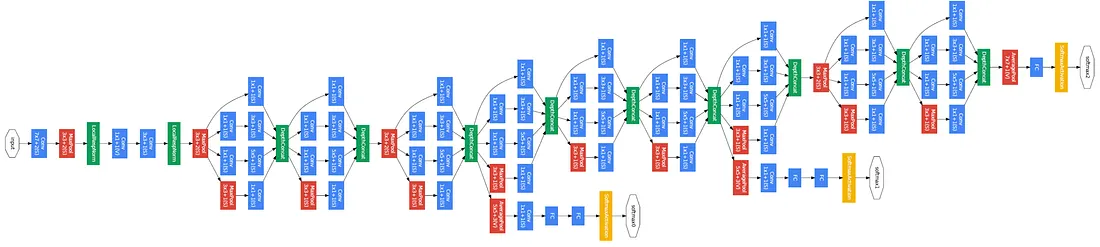
\includegraphics[width=\textwidth]{chapters/03-cnn/media/GoogLeNet.png}
    \caption{GoogLeNet architecture.}
    \hfill
\end{figure}

\paragraph{Inception Modules}
The Inception Module is a fundamental building block of the GoogLeNet architecture. 
It is designed to allow the network to learn multiple types of features at different scales, while keeping the number of parameters manageable.
Instead of choosing a single filter size, the module applies $1 \times 1$, $3 \times 3$, and $5 \times 5$ convolutions, along with a $3 \times 3$ max-pooling operation, in parallel.

This approach offers two primary advantages:
\begin{itemize}
    \item \textbf{Multiscale Feature Extraction:} It allows the network to automatically decide which filter size is most relevant for a given feature, effectively handling objects of varying sizes within the ImageNet dataset.
    \item \textbf{Feature Redundancy and Generalization:} Reusing the same input across parallel paths enforces a degree of redundancy in the learned feature maps. This redundancy encourages the model to learn more robust, scale-invariant representations, which significantly improves the generalization performance and provides a regularizing effect during training.
\end{itemize}
The outputs of all these operations are then concatenated together to produce the output feature map of the module.

\begin{figure}[H]
    \centering
    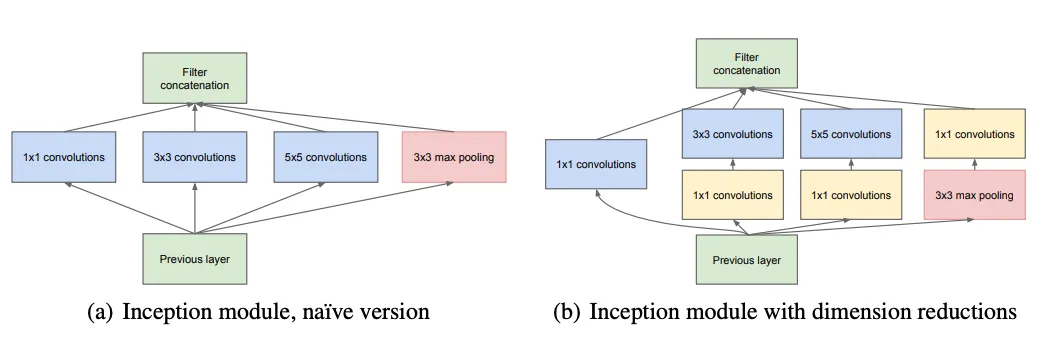
\includegraphics[width=\textwidth]{chapters/03-cnn/media/inceptionModule.png}
    \caption{Inception Module.}
\end{figure}

\subsubsection{ResNet (2015)}
As architectures grew increasingly deep, researchers encountered the \textbf{degradation problem}: as network depth increases, 
accuracy begins to saturate and then degrades rapidly. 
Crucially, this degradation is not caused by overfitting, as it is characterized by higher \textbf{training error} than their shallower counterparts.

ResNet, introduced in 2015, addressed this issue by introducing the concept of \textbf{residual connections} (or skip connections), 
which allows the network to learn to skip certain layers if they are not useful for the task at hand, 
effectively allowing the network to learn an identity mapping (i.e., the input is passed through unchanged) if needed.

It was shown that this simple architectural provided various benefits, such as:
\begin{itemize}
    \item \textbf{Implicit Ensemble Learning:} The skip connections allow the network to learn multiple paths for information flow, 
    effectively creating an ensemble of shallower networks within the deeper architecture. 
    \item \textbf{Smoother Loss Landscape:} The skip connections help to smooth the loss landscape, making it easier for 
    the optimization algorithm to find a good solution and improving convergence during training.
\end{itemize}

\paragraph{Dimensions mismatch}
It's important to note that not always the skip connections could be used, due to dimension mismatch between the input and output of the layers.
To resolve this issue, the concept of $1 \times 1$ convolution was reused, allowing to match the dimensions of the input and output feature maps, 
while also providing an additional level of feature transformation.

\paragraph{Different residual blocks} 
In the later years, different types of residual blocks were proposed. Instead of identity skip connections, some architectures used more 
complex transformations in the skip connections, such as:
\begin{itemize}
    \item \textbf{Pre-activation Residual Block}: the order of batch normalization and activation functions is changed, to precede the
    final convolution. This creates a cleaner identity mapping, as the skip connection is not affected by the non-linear transformations, 
    and allows for better gradient flow during training;
    \item \textbf{Bottleneck Residual Block}: this block uses a $1 \times 1$ convolution to reduce the number of channels before applying the expensive $3 \times 3$ convolution,
    and then uses another $1 \times 1$ convolution to restore the original number of channels after the convolution operation.
    \item \textbf{Wide Residual Block}: focuses on increasing the width of the network (i.e., the number of channels) instead of the depth, by applying wider convolutional 
    layers and using fewer layers overall. This approach allowed to investigate the trade-off between depth and width in CNNs, to find the optimal trade-off for different tasks and datasets.
\end{itemize}
Following the success of ResNet, many architectures were proposed that built upon the idea of residual connections. 
The next 2 architectures we will briefly describe are examples of this trend.

\subsubsection{DenseNet (2018)}
DenseNet are a type of CNN architecture that builds upon the idea of residual connections. Instead of using skip connections that add the input to the output of a layer, 
DenseNet introduces the \textbf{Dense Block}. 

In a Dense Block, each layer is connected to all the other layers that compose the block. This means that for each layer, the feature maps of
all the previous layers are concatenated together and used as input for the current layer.

This approach has a few advantages, such as:
\begin{itemize}
    \item \textbf{Feature Reuse:} Since feature maps are preserved via concatenation, there is no need to relearn redundant features in subsequent layers.
    \item \textbf{Parameter Efficiency:} Despite the dense connectivity, DenseNets often require fewer parameters than ResNets for similar performance because they do not need large, wide layers to capture complex information.
\end{itemize}

\subsubsection{SENet (2019)}
SENet (Squeeze-and-Excitation Networks) is a type of CNN architecture that introduces the concept of \textbf{channel attention}. 
Channel attention allows the network to learn to focus on the most important channels of the feature maps, by applying a weighting 
mechanism to the channels based on their importance for the task at hand.

The SE block learns to emphasize informative channels and suppress less useful ones, effectively allowing the network to adaptively recalibrate channel-wise feature responses.
This is achieved through a two-step process:
\begin{itemize}
    \item \textbf{Squeeze}: Global average pooling is applied to the input feature, producing an average representation of each channel;
    \item \textbf{Excitation}: Using a sigmoid activation function, the network learns to generate weights for each channel. 
\end{itemize}
The output of the SE block is obtained by multiplying the input feature maps by these learned weights, effectively emphasizing important channels and suppressing less useful ones.

\subsubsection{ConvNext (2022)}
In the later years, the trend of transformer-based architectures has dominated the field of computer vision, with models such as \textbf{Vision Transformer (ViT)} and \textbf{Swin Transformer} 
achieving state-of-the-art performance on various vision tasks.

ConvNext is a CNN architecture that was proposed in 2022. It showed that with some modifications to the standard CNN architecture, it is possible to achieve performance 
comparable to transformer-based architectures, while still maintaining the efficiency and simplicity of CNNs.

\subsection{Regularization}
To prevent overfitting, various regularization techniques were developed specifically for CNNs, such as:
\begin{itemize}
    \item \textbf{Cutout}: this method involves randomly masking out a square portion of the input image during training, replacing it with the mean pixel value of the dataset.
    This approach forces the network to learn more robust features that are not reliant on specific parts of the image;
    \item \textbf{DropBlock}: an extension of dropout, where instead of randomly dropping individual neurons, contiguous regions of the feature maps are dropped during training,
    for all channels.
    \item \textbf{CutMix}: this method involves randomly cutting and pasting patches between training images.
    Class labels are also updated proportionally to the area of the patches. This encourages the model to learn features from different parts of the images,
    providing a regularization effect and improving generalization.
\end{itemize}

